\documentclass{bioinfo} 
\copyrightyear{2016} \pubyear{2016}
\access{Advance Access Publication Date: Day Month Year}
\appnotes{Original Paper} 
\usepackage{amsmath, amssymb}
  \allowdisplaybreaks % YEAH!
\usepackage{textcomp} 
%\usepackage[
%    colorlinks, linkcolor={blue}, citecolor={blue},
%    urlcolor={red}]
%{hyperref}
%\renewcommand*{\HyperDestNameFilter}[1]{}
%% Option 1 URW Garamond (free any latex distribution): 
%% ====================
%    \usepackage[urw-garamond]{mathdesign} 
%    \usepackage[T1]{fontenc}
%% Option 2: Classic Garamond (requires .pfb sources)
%% ==========================
    \usepackage[T1]{fontenc}
    \usepackage{sabon}
    \usepackage[italic,defaultmathsizes]{mathastext}
    % mdugm.sty magic bellow --!!!
    \SetSymbolFont{letters}{normal}{OML}{mdugm}{m}{it} 
%% Option 3 (Times via MathTimes Pro)
%% =================================
%    \usepackage[subscriptcorrection]{mtpro}
%       \DeclareMathSizes{8}{7.15}{5.2}{4.2}
%    \usepackage[mtpcal]{mtpb}
\DeclareMathAlphabet{\txcal}{U}{tx-cal}{m}{n}
\usepackage[scaled=1.1]{rsfso}
\renewcommand*\ttdefault{txtt}
%
\usepackage{microtype}
%
\newcommand{\wP}{P^\ast}
\newcommand{\wE}{E^\ast}
\newcommand{\wZ}{Z^\ast}
\newcommand{\wt}{\theta^\ast}
\newcommand{\wk}{\psi^\ast}
\newcommand{\whp}{\widehat \pi}
\newcommand{\wAe}{A_e^\ast}
\newcommand{\wAp}{A_p^\ast}
\newcommand{\wBe}{B_e^\ast}
\newcommand{\wBp}{B_p^\ast}
\renewcommand*\copyright{\textcopyright}
\newcommand{\CC}{C\nolinebreak\hspace{-.05em}\raisebox{.4ex}{\tiny\bf
    +}\nolinebreak\hspace{-.10em}\raisebox{.4ex}{\tiny\bf +}} 
\begin{document}
\firstpage{1}
%\subtitle{}
\title[empirical Bayesian NMF]{An empirical Bayesian approach to
  mutational signature discovery}
\author[Rosales, R. A. and Drummond, R. D.~\textit{et~al}.]{
    R. A. Rosales\,$^{\text{\sfb 1,}\dagger}$, 
    R. D. Drummond\,$^{\text{\sfb 2,}\dagger}$, 
    R. Valieris\,$^{\text{\sfb 2}}$,  and
    I. T. da Silva\,$^{\text{\sfb 2,3}*}$} 
\address{%
   $^{\text{\sf 1}}$Departamento de Computa\c{c}\~ao e
   Matem\'atica, Universidade de S\~ao Paulo, 14040-901 SP, Brazil\\ 
   $^{\text{\sf 2}}$Laboratory of Bioinformatics and Computational 
   Biology, CIPE/A.C. Camargo Cancer Center, S\~ao Paulo  01509-010, 
   Brazil\\
   $^{\text{\sf 3}}$Laboratory of Molecular Immunology, The
   Rockefeller University, New York, NY 10065, USA\\[1em]
   {\normalsize $^{\dagger}$The authors wish it to be known
     that, in their opinion, the first two authors should be regarded
     as joint First Authors} 
}
\corresp{$^\ast$To whom correspondence should be addressed.} 
\history{Received on XXXXX; revised on XXXXX; accepted on XXXXX} 
\editor{Associate Editor: XXXXXXX} 
\abstract{%
 \textbf{Motivation:} Analysis of somatic mutations.\\
 \textbf{Results:} Developed a full (empirical) Bayesian treatment to
the factorisation problem.\\
 \textbf{Contact:}
%\href{rrosales@usp.br}{\texttt{rrosales@usp.br}},
%\href{rdrummond@gmail.com}{\texttt{rdrummond@gmail.com}},
%\href{rvalieris@gmail.com}{\texttt{rvalieris@gmail.com}},
 itojal@gmail.com\\
\textbf{Supplementary information:} Supplementary data are available 
at \textit{Bioinformatics} online.
}
\maketitle
\section{Introduction}
Cancer is an evolutionary process driven by continuous acquisition of
heritable genetic variations in individual cells. A set of acquired
mutations in cancer cells allows a growth advantage over its neighbour
cells, thereby triggering the expansion of the tumor cell clone. The
diversity and complexity of somatic mutational processes in these
clones is a conspicuous feature orchestrated by DNA damage agents and
repair processes, including exogenous or endogenous mutagen exposures,
defects in DNA mismatch repair and enzymatic modification of DNA,
\cite{RG}. The actual identification of the underlying mutational
processes is central to understanding of cancer origin and evolution,
\citealp{RG, AS, HEN}.
% RR: I will elaborate on this next phrase below:
%Nowadays, few computational approaches have been developed to
%extract the repertoire of mutational signatures and processes
%operating across the cancer genome \citealp{NCell, FICMV}.


Somatic mutations usually consist of single base substitutions that
fall into one of six possible base changes, namely
\texttt{C:G}$>$\texttt{A:T}, \texttt{C:G}$>$\texttt{G:C},
\texttt{C:G}$>$\texttt{T:A}, \texttt{T:A}$>$\texttt{A:T},
\texttt{T:A}$>$\texttt{C:G} and \texttt{T:A}$>$\texttt{G:C}. According
to \cite{A}, this set may be further enlarged by including the $5'$
and $3'$ neighbouring bases of each substitution site, leading to an 
alphabet $\txcal A$ with 96 trinucleotide mutation types. More
generally, the definition of $\txcal A$ could in principle accommodate
mutations of various other kinds such as indels, rearrangements, copy
number changes and even wider neighbouring contexts. Once $\txcal A$
is properly defined, the counts for the mutations found in $G$
different genomes are assembled into a $K\times G$ matrix $M$ with $K
= |\txcal A|$. A key assumption consists in viewing the counts in $M$
as the additive effect of $N$ mutational processes, each defined as a
$K\times 1$ vector of mutational rates. The later defines what
is known to be as a mutational signature. More precisely, the
mutations across all genomes result as the linear combination of $N$
basis vectors of dimension $K\times 1$, with mixture coefficients
defined by $N$ exposure vectors of dimension $1 \times G$. If the
basis vectors are merged into a $K\times N$ matrix of signatures $P$,
and the coefficient vectors into a $N\times G$ matrix of exposures
$E$, then the data can be simply factored as $M=PE$. An example of
this procedure is shown in Figure~\ref{fig:toyNMF}.

\begin{figure*}
 \centering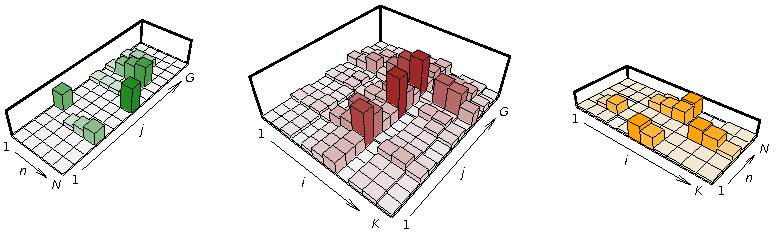
\includegraphics[width=15cm]{figs/f}
 \caption{\textrm{%
  A factorisation for a mutation counts matrix $M$. The
mutation matrix shown at the left is defined over an alphabet with
$K=11$ symbols, $1 \leqslant i \leqslant 11$, and $G=15$ genomes,
$1\leqslant j\leqslant 15$. The matrices at the centre and the right
represent respectively a signature matrix $P$ and an exposure matrix
$E$ for a factorisation with rank $N=5$.
  }
 }
\label{fig:toyNMF}
\end{figure*}

For a given a matrix of observed mutation counts there are essentially
two interrelated questions that should be addressed. The first one
concerns the determination of the underlying signatures and their
exposures to best account for the observations. The second is related
to the determination of the actual number of signatures,
$N$. \cite{NCell} and \cite{A} addressed the first issue by using
nonnegative matrix factorisation (NMF) techniques.  NMF as conceived
by \cite{LS} finds the factors $P$, $E$ that approximately solve the
following non-convex optimisation problem
\begin{equation}
 \label{eqn:NMF}
  \min_{P\geqslant 0,\ E\geqslant 0}\|M - PE\|,
\end{equation}
for a given fixed rank $N$ and an appropriately chosen matrix norm
$\|\ \|$.  In order to deal with the second question, \cite{NCell} and
\cite{A} perform the factorisation of the same data for various
values of $N$ ranging from 1 to $\min\{K, G\}-1$. The rank is then
determined rather indirectly by studying the clustering properties of
the obtained factors via a criterion developed by \cite{BTGM} or by 
using the residual sum of squares, \cite{HMSG}.


An alternative approach to mutational signature discovery, and to NMF
in general, follows from a statistical interpretation of the problem
posed by (\ref{eqn:NMF}) in which $M$ is assumed to be a random matrix
distributed according to a member of the exponential family
parameterised by $P$ and $E$. The optimisation problem posed by
(\ref{eqn:NMF}), under the norm induced by a specific Bregman
divergence (see \citealp{BMD}), turns to be equivalent to the maximum
likelihood estimation of $P$ and $E$.  For instance, if $M$ is Poisson
distributed with rate $PE$, then the likelihood maximisation with
respect to $P$ and $E$ is equivalent to the minimisation of
(\ref{eqn:NMF}) under the norm defined by the Kullback-Leibler
divergence. The maximisation of a Gaussian likelihood is equivalent to
the minimisation under the Frobenius norm. A key aspect of this
perspective is that it allows to treat the determination of the
factorisation rank $N$ as a model selection problem. The statistical
interpretation was developed by \cite{C}, \cite{FC} and \cite{SWK} in
the general NMF context and then considered by \cite{FICMV} for the
mutational signature application. \cite{FICMV} modelled $M$ as Poisson
distributed and then considered the estimation of $P$ and $E$ by using
an expectation maximisation (EM) algorithm. The number of mutational
signatures where estimated by considering an (unnecessary) saddlepoint
approximation to Bayesian information criterion (BIC).


% Both of these models correspond to the ones initially considered by
% \cite{LS} from the optimisation perspective. The latter is in fact
% the one implemented by \cite{A}. The statistical perspective to NMF
% was observed and then further developed by by \cite{C}, and
% \cite{FC}. A key observation of the statistical approach is that it
% allows to cast the determination of the NMF rank formally as a model
% selection problem. In this regard, \cite{FICMV} considered the
% estimation of mutational signatures under the Poisson model by
% estimating $P$ and $E$ by an instance of the Expectation
% Maximisation (EM) algorithm, that happens to be be identical to the
% optimisation method in \cite{LS}. The NMF model order is chosen by
% using the Bayesian information Criterion (BIC).


%\cite{NCell} introduce a multivariate analysis technique,
%termed non-negative matrix factorisation (NMF) to extract mutational
%signatures in the genomes of 21 breast cancers. In a later work, they
%also explored the heterogeneity of mutation signature within cancer
%types \cite{ANat}. More recently, \cite{FICMV} propose an explicitly
%probabilistic framework to infer the number of elementary mutational
%processes  and their spectra from cancer sequence data. This method
%allows the  tumor-specific opportunity for different mutation types
%according  to sequence composition, which is particularly important to
%account  for biases in the mutational opportunity and to accommodate
%noisy  data \cite{FICMV}.

\section{Approach}
\subsection{Hierarchical model}
\subsubsection{Likelihood and latent variables}
Let $p_{in} = (P)_{in}$ be the $i,n$-entry of $P$. Likewise let
$e_{nj} = (E)_{nj}$ and $w_{ij} = (W)_{ij}$.  The mutation counts
$(M)_{ij}$ are assumed to be Poisson distributed random variables with
rates $(PE)_{ij}(W)_{ij} = w_{ij}\sum_{n=1}^N p_{in}e_{nj}$. For a
given sample of $M$, say $m$, this formulation is sufficient to define
the likelihood function $\mathcal L(\theta; m)$ if one identifies the
matrices $P, E$ as model parameters $\theta$ with $\theta \in \Theta =
\mathbb R_+^{K\times N}\times \mathbb R_+^{N\times G}$. An expression
for $\mathcal L(\theta; m)$ is presented in ($s_1$). This relatively
simple model allows for a latent variable representation in which the
observed counts are expressed as the sum of $N\geqslant 1$ independent
Poisson variables
\begin{equation}
  \label{eqn:latent_representation}
   M_{ij} = Z_{i1j} + Z_{i2j} + \ldots + Z_{iNj},
\end{equation}
each with rate respectively equal to $p_{in}e_{nj}w_{ij}$. This
description is an immediate consequence of the properties of sums of
independent Poisson random variables. Biologically, this accounts for
the observation that the total number of mutations of a specific type,
say $i,j$, arise as the linear combination of $N$ mutational processes
$Z_{inj}$, $n = 1, \ldots, N$. From a statistical perspective,
(\ref{eqn:latent_representation}) enables a data augmentation scheme
that becomes instrumental for a Bayesian treatment to NMF, allowing
the implementation of Expectation Maximisation (EM), Markov chain
Monte Carlo (MCMC), and variational Bayes approximations, see
\cite{C}.  Hereafter let $Z = \{Z_{inj}: 1\leqslant i\leqslant K,
1\leqslant n \leqslant N, 1\leqslant j\leqslant G\}$, and $z =
\{z_{inj}\}$ denote a generic value for $Z$.


\subsubsection{Priors} 
We consider conjugate priors for the matrices $P$ ans $E$ by modeling
each of their entries as a Gamma distributed random variable.
Specifically, $p_{in}$ has a Gamma distribution with shape
$\alpha_{in}^p + 1$ and rate $\beta_{in}^p + \delta_e$, for
$\alpha_{in}^p \geqslant 0$, $\beta_{in}^p \geqslant 0$. Likewise,
$e_{nj}$ are Gamma distributed with shape $\alpha_{nj}^e+1$ and rate
$\beta_{nj}^e + \delta_e$, for $\alpha_{nj}^e \geqslant 0$,
$\beta_{nj}^e \geqslant 0$. Shape parameters are shifted by 1 to
ensure bounded values for the Gamma densities\footnote{RD: we need to
explain this. That is, why do we have to avoid a `singularity' near
the origin?}. The rate parameters are shifted by $\delta_p \geqslant
0$ and $\delta_e \geqslant 0$ to prevent arbitrarily large values for
the elements of $P$ and $E$\footnote{RD: same here, I think we have to
explain. We have to mention that these choices are not too stringent
(too informative).}. Denote by $A_p$ and $B_p$ be $K\times N$ matrices
respectively with entries $\alpha_{in}^p$ and $\beta_{in}^p$, and
$A_e$, $B_e$ be $N\times G$ matrices with elements $\alpha_{nj}^e$ and
$\beta_{nj}^e$. Let $\psi = (A_p, B_p, A_e, B_e)$ be a vector formed
by the full set of hyperparameter matrices, that is the parameters of
the prior distributions.

\subsubsection{Hyperpriors} 
A further hierarchy in our model is set by considering the
distributions for the hyperparameters $\psi$\footnote{RR: Maybe we
have to justify why all this was made. The reason is to reduce the
dependency on a large number of free hyperparameters for the model
choice approach, i.e. the marginal likelihood depends upon the actual
values of the hyperparameters if we don't integrate them out: for
$N=5$, $G=21$, $K=96$ we have $2(KN+NG)=1170$ (hyper)parameters to
set. With the hierarchical model, we are able to reduce the free
parameters down to 6.}. By conjugancy to the prior, we
define the entries of $B_p$ as being independent and distributed
according to a common Gamma distribution with known shape and rate
$a_p > 0$, $b_p > 0$. Similarly, the elements of $B_e$ are Gamma
distributed with the same shape $a_e>0$ and rate $b_e>0$. For the
$A_p$ and $A_e$ hyperparameter matrices the situation is
different. While a Gamma distribution for the entries of $A_p$ and
$A_e$ is conjugate to the Gamma prior (see \citealp{M}), the resulting
full conditional distribution necessary in order to draw inferences
about $A_p$ and $A_e$ does not has a standard form.  This fact has
long been recognized in the Poisson hierarchical model
(\citealp{GMS93}) and may be dealt with by choosing any parametric
family of probability distributions with the appropriate support. Here
we consider the elements of $A_p$ and $A_e$ as independent and
exponentially distributed with rates $\lambda_p > 0$ and $\lambda_e >
0$.  Let $\eta$ be the vector of hyperprior parameters $\eta = (a_e$,
$b_e$, $a_p$, $b_p$, $\lambda_p$, $\lambda_e) \in \Lambda = \mathbb
R_+^6$.
% $\psi \in \Psi = \mathbb R_+^{K\times N}\times \mathbb R_+^{N\times
% G}\times \mathbb R_+^{K\times N}\times\mathbb R_+^{N\times G}$ and
% $z \in \txcal Z = \mathbb Z_+^{K\times N\times G}$.

\subsection{Bayesian treatment}
We consider an empirical Bayesian approach in which the parameters
$\theta$, the hyperparameters $\psi$ and the hyperprior parameters
$\eta$ are all estimated from the data.  Inferences are driven from
the conditional posterior $\pi(\theta|M, \eta)$ by combining
Markov chain Monte Carlo (MCMC) and Expectation Maximisation (EM)
techniques as encouraged by \cite{C01} or \cite{LC}. Specifically, a
(Metropolized) Gibbs sampler targeted towards the conditional
posterior $\pi$ is constructed in order to generate a sequence of
samples $\{Z^{(r)}, \theta^{(r)}, \psi^{(r)}\}$, $r = 1, \ldots,
R$. This sequence is the used to obtain an estimate for the marginal 
posterior $\pi(\theta|M, \eta)$, 
\[
   \hat{\pi}(\theta|M, \eta) 
 = 
   \frac{1}{R}\sum_{r=1}^R \pi(\theta|Z^{(r)}, \psi^{(r)}, M, \eta). 
\]
which is then used to drive all subsequent inferences concerning
$\theta$, the mutational signatures and their exposures.

This sequence is the used to obtain $\hat\eta$, an estimate of
$\eta$ by using a Monte Carlo EM algorithm. An eventual run of the
sampler with $\eta$ fixed at $\hat\eta$ is then used to estimate the
NMF factors $\widehat P$ and $\widehat E$ and any other associated
posterior statistic. The output generated by the MCMC analysis is also
considered to estimate the NMF factorisation rank, namely the NMF
model order by considering the computation of marginal
likelihoods. Details about the Gibbs sampler are relatively standard
and thus included as supplementary material. The following two
sections focus on the Monte Carlo EM technique and the general
Bayesian model selection approach adopted here. A subsequent section
presents the actual algorithm used to make all inferences.

\subsubsection{MCMC EM}\label{sec:MCMCEM}
For a given data sample $m$, direct use of Bayes theorem
allows to  express the the marginal likelihood for $\eta$, i.e. the
function $\mathcal L: \Lambda \to \mathbb R_+$ induced by the map $\eta 
\mapsto p(M=m|\eta)$, as
\begin{equation}
  \label{eqn:margLik}
  \mathcal L(\eta; m) 
  = p(m, Z, \theta, \psi\,|\,\eta)\,\big/\pi(Z,
      \theta, \psi|m, \eta).
\end{equation}
Similarly, let $\mathcal L(\eta; m, Z, \theta, \psi)$ equal the
distribution $p(M=m$, $Z$, $\theta$, $\psi|\eta)$, but considered as a
function of $\eta$. Taking\footnote{RR: explain what is what, in FULL
  LENGTH} logarithms and integrating with respect to the posterior  distribution  $\pi(Z,  \theta, \psi|m,  \eta)$ with $\eta = \eta_0$ gives 
\begin{align*}
   \mathbb E\big[\ln\mathcal L(\eta; m) \big| \eta_0\big] 
  =& 
  \mathbb E\big[\ln\mathcal L(\eta; m, Z, \theta, \psi)
    \big|  \eta_0\big]\\ 
  &-
  \mathbb E\big[\ln \pi(Z, \theta, \psi\,|\,m,\eta)\big| \eta_0\big].
\end{align*}  
This expression is the basic identity on which the EM algorithm is
built and justifies therefore the convergence of the sequence
\begin{equation}
 \label{eqn:EofMCEM}
  \eta^{(k+1)} = \underset{\eta\,\in\, \Lambda}{\text{arg max}}\, 
  \mathbb E\Big[\ln\mathcal L(\eta; m, Z, \theta, \psi)\big|
  \eta^{(k)}\Big], 
  \quad k\geqslant 0,
\end{equation}
towards the maximum likelihood estimate of $\eta$ for any $\eta^{(0)}
= \eta_0  \in \Lambda$. The integral involved in the above expectation
cannot be computed directly but it may be estimated via Monte Carlo,
leading to the sequence 
\begin{equation}
 \label{eqn:MCEM}
   \hat\eta^{(k+1)}
 = 
    \underset{\hat\eta^{(k)}\,\in\,\Lambda}{\text{arg max}} 
   \bigg\{
    \frac{1}{R}\sum_{r=1}^R 
      \ln\mathcal L\Big(\hat\eta^{(k)}; m, Z^{(r)}, \theta^{(r)},
      \psi^{(r)}\Big)
   \bigg\}.
\end{equation}



This procedure is valid because the MCMC sampler developed throughout
generates $\{Z^{(r)}, \theta^{(r)}, \psi^{(r)}\}$, $r = 1,
\ldots, R$, approximately from the posterior distribution that is
actually used to define the expectation in (\ref{eqn:EofMCEM}). The maximisation steps involved in (\ref{eqn:MCEM}) are relatively
simple to implement and further detailed as supplementary material. 


This rises however the issue as to in what sense $\hat\pi(\theta|M,
\hat\eta)$ can be regarded as an estimate for the posterior 
$\pi(\theta|M, \eta)$. The answer to this is provided by the following
result, which ensures the convergence of the statistic. For any
measurable set $T\subseteq \Theta$, it follows that
\[
   \lim_{R,\ k\to\infty}
     \int_T \frac{1}{R}
    \bigg|
       \sum_{r=1}^R \pi(\theta|M, \psi^{(r)}, Z^{(r)}, 
          \hat\eta^{(k)}) - \pi(\theta|M,\eta)
    \bigg|\ d\theta = 0.
\]
This result is formally stated as Theorem 1 and further proved in the
accompanying supplementary material.




%%%\end{methods}

\subsection{Parameter estimation}
The algorithm to estimate $\eta$ and generate the samples for $(Z,
\theta, \psi)$ conditionally upon the estimate for $\eta$ proceeds as 
follows. 
\begin{enumerate}
\item[\textbf{1}.] Set $k = 0$ and initialise $\eta^{(k)}$.
\item[\textbf{2}.] Initialise $Z^{(0)}$, $\theta^{(0)}$, $\psi^{(0)}$
  by sampling $\psi$ from $p(\psi|\eta^{(0)})$, the model hyperprior,
  and then $\theta$ from $p(\theta|\psi)$, the model prior. Optionally
  $\theta^{(0)}$ may be initialised by solving (\ref{eqn:NMF})
  via the NMF package from within R, see \citealp{GS}. 
\item[\textbf{3}.] Iterate the Gibbs sampler to generate the sequence
$\{Z^{(r)}, \theta^{(r)}, \psi^{(r)}\}$, $r = 1, \ldots, R$.
\item[\textbf{4}.] Update $\hat\eta^{(k)}$ with the Monte Carlo EM
formula in (\ref{eqn:MCEM}) and set $k = k+1$. Return to step
\textbf{3} until $\big\|\hat\eta^{(k)} - \hat\eta^{(k-1)}\big\|_\infty 
\leqslant 0.05$ or $k > 100$. 
\item[\textbf{5}.] Set $\hat\eta = \hat\eta^{(k)}$ and then generate a 
  final realization of the Gibbs sampler, producing the sequence of
  samples $\{Z^{(r)}, \theta^{(r)}, \psi^{(r)}\}$, $r=1, \ldots
  R$. 
\end{enumerate}

The final sequence of samples generated in step \textbf{5} is used to
compute point estimates for $P$ and $E$ as $\widehat P =
R^{-1}\sum_{r=1}^R P^{(r)}$, and $\widehat E = R^{-1}\sum_{r=1}^R
E^{(r)}$. Further posterior statistics such as the NMF factors
variances or coverage intervals are also obtained from this
sample.\footnote{RD: this may be the place to further comment on your
ideas.}



\section{Methods}
\subsection{Data} The data set containing 183916 somatic point
mutations from 21 breast cancer genomes was obtained from
\verb+ftp://ftp.sanger.ac.uk/+ \verb+pub/cancer/Nik-ZainalEtAl+, by
following the instructions in Table S1 in~\cite{NCell}. Single base 
substitutions where mapped onto trinucleotide sequences by considering
the $5'$ and $3'$ neighboring bases in order to construct a $96\times
21$ matrix of mutation counts $M$. 
%\footnote{IT, RD, RV: What is the
%appropriate way to reference this?  Some papers (by
%Nik-Zainal/Alexandrov) point to COSMIC
%(\verb+http://www.sanger.ac.uk/genetics/CGP/cosmic+), but I have not
%been able to find the data there! The ftp link here was found in
%Table S1 of \cite{NCell}. DO CHECK.}. 
The opportunity matrix $W$ was constructed (or taken from) ...


\subsection{\texttt{signeR}} Describe R's package
source destination. Mention that is has been optimized in
\CC. A detailed explanation about how to install, run, etc is
presented as supplementary material.

\section{Results}
\subsection{21 breast cancer data}
Include the 21 breast cancer data and simulated data. For the latter,
I was thinking on simulating with $G=20$ and $K=5$, with signatures
of  our myeloma data. 
%\begin{figure}
% \centering\includegraphics[width=8.5cm]{Signatures_gold_standard}
% \caption{\textrm{% 
%    A factorization for the 21 breast cancer data set. 
%  }
% }
%\label{fig:bcancerNMF}
%\end{figure}


The results for the BIC evaluated at the samples generated via MCMC at 
step 5 for $1 \leqslant N \leqslant 12$ are shown in Figure~*. The BIC
at $\theta^{(r)}$, is computed as
$
 \text{BIC}(\theta^{(r)}) = 2\ln\mathcal L\big(m; \theta^{(r)}\big) -
     N(G+K)\ln G.
$

\subsection{Simulation study}
To further asses the reliability of our methods we considered the
analysis of synthetic data. To this end we took the mutational
signatures 2, 3, 13 and 17 found in , found in most breast cancer genomes.


\section{Discussion}
The idea that many cancers acquire a mutational phenotype\footnote{IT:
was \emph{mutator phenotype}; Still we have to improve} at different
intensities is well accepted. Therefore, the ability to detect 
mutational signatures may provide insights about the development of
tumours. Here, we have outlined signeR, it employs a different and 
novel approach to deciphering mutational signatures, and featuring a
number of advantages when compared with others approaches. First, it
xxx. . Second, xxx and Third ....


Send a final message but don't be repetitive.


\section*{Funding}
This work was partially supported by the grant $\ldots$ (FAPESP). 
\vspace*{-12pt}
 
%\bibliographystyle: natbib, achemnat, plainnat, abbrv, plain 
\bibliographystyle{bioinformatics}
\bibliography{bnmf}
\end{document} 

%%% Local Variables:
%%% mode: latex
%%% TeX-master: t
%%% End: